\documentclass[conference]{IEEEtran}
\IEEEoverridecommandlockouts
% The preceding line is only needed to identify funding in the first footnote. If that is unneeded, please comment it out.
\usepackage{cite}
\usepackage{amsmath,amssymb,amsfonts}
\usepackage{algorithmic}
\usepackage{graphicx}
\usepackage{textcomp}
\usepackage{xcolor}
\usepackage{hyperref}

\def\BibTeX{{\rm B\kern-.05em{\sc i\kern-.025em b}\kern-.08em
    T\kern-.1667em\lower.7ex\hbox{E}\kern-.125emX}}
\begin{document}

\title{Centralized Composable HPC Management with the OpenFabrics Managment Framework\thanks{Sandia National Laboratories is a multi-mission laboratory managed and operated by National Technology \& Engineering Solutions of Sandia, LLC, a wholly owned subsidiary of Honeywell International Inc., for the U.S. Department of Energy’s National Nuclear Security Administration under contract DE-NA0003525.}\thanks{The OpenFabrics Alliance (OFA) mission is to accellerate the development and adoption of advanced fabrics for the benefit of the advanced networks ecosystem, which is accomplished by: creating opportunities for collaboration among those who develop and deploy such fabrics, incubating and evolving vendor independent open source software for fabrics, and supporting and promoting the use of such fabric technology software.}
}

\author{\IEEEauthorblockN{1\textsuperscript{st} Michael Aguilar}
\IEEEauthorblockA{\textit{High Performance Computing Systems} \\
\textit{Sandia National Laboratories}\\
Albuquerque, New Mexico, USA \\
mjaguil@sandia.gov}
\and
\IEEEauthorblockN{2\textsuperscript{nd} Phil Cayton}
\IEEEauthorblockA{\textit{Senior Staff Engineer} \\
\textit{Intel Corporation}\\
Hillsboro, Oregon, USA \\
phil.cayton@intel.com}
\and
\IEEEauthorblockN{3\textsuperscript{rd} Michele Gazetti}
\IEEEauthorblockA{\textit{Research Engineer} \\
\textit{IBM Research Europe}\\
Dublin, Ireland\\
Michele.Gazzetti1@ibm.com}
\and
\IEEEauthorblockN{3\textsuperscript{rd} Russ Herrell }
\IEEEauthorblockA{\textit{EE system architect at Hewlett-Packar} \\
\textit{Hewlett Packard Enterprise}\\
Fort Collins, CO, USA\\
rherrell@hpe.com}
}

\maketitle

\begin{abstract}
Current HPC systems are limited in performance and architecture by the the stranding of disaggregated components. In current HPC systems, common tools do not exist to manage increasingly diverse network fabrics and component resources, such as, CPUs, hierarchical memory components, remote NVMe, and accelerators.  Due to lack of access to good Resource Management tools, current HPC systems suffer from inefficient over-design where resources must be provided locally, often in node, to make In instances that HPC running jobs could potentially require the resources.  In addition, the inability to dynamically share available resources, as they are required by running batch jobs can lead to reduced and inefficient computational performance and running job failure.  Centralized resource management can potentially mitigate, out-of-memory conditions, IO thashing, stranding of available resources, such as, CPUs, GPUs, and memories, and provide dynamic network fail-over.  It is clear that Resource Management, using a standardized interface, can enable clients to monitor, compose, and intelligently provision resources, in beneficial ways.

The OpenFabrics Management Framework (OFMF) is a open-source Resource Manager being developed by the OpenFabric Alliance (OFA), the DMTF, SNIA, and the CXL Consortium. The OFMF implements Redfish and Swordfish through the implementation of a Swordfish Endpoint Emulator and network Agents.  The Emulator provides centralized resource monitoring and command control for the attached hardware resources and network fabrics, through matching network Agents. A Composability Manager, integrated with the OFMF, can mitigate stranded resources by providing a method for sharing hardware, CPUs, GPUs, NVM, and memories.  Integration with the OFMF provides the capability for dynamic provisioning of resources to maintain running client computations.  

The OFMF is designed for configuring fabric interconnects and managing composable disaggregated resources in dynamic HPC infrastructures using client-friendly abstractions.  The goal of the OFMF is to enable interoperability through common interfaces to enable client Managers to efficiently connect workloads with resources in a complex heterogenous ecosystem without having to worry about the underlying network technology.  

In addition, the OFMF project scope includes adding functional components to manage e.g., Network, GPU, and CPU Composition, Fabric Attached Memory, Fabric Attached Storage, Platform Composition, and Monitoring. 
\end{abstract}

\begin{IEEEkeywords}
component, formatting, style, styling, insert
\end{IEEEkeywords}

\section{Introduction}

Traditional HPC compute clusters are created by combining separate compute servers over network fabric devices to form the cluster.  Each individual compute server is provisioned with its own CPUs, memory devices, accelerator cards, and storage devices to incorporate as many different application runtime requirements as possible.<cite >. This need to incorporate 'all of the options' makes traditional HPC architectures less flexible, inefficient, and can lead to situations where application jobs more prone to run-time failure.    
For example, design considerations that lead to an under-estimation of compute server memory resources can cause out-of-memory conditions.  In another example, IO server memory oversubscription can result in filesystem failure can occur due to virtual memory page swap thrashing and eventually application failure when the dynamic addition of memory would be able to help mitigate this problem.  

Yet another issue with current HPC architecture that is a result of architectural inflexibility frequently results in overprovisioned or stranded resources.  Stranded resources are defined as resources that are either on a compute server that is unavailable to a workload, or that have been assigned to a workload that isn't making use of them.  These resources have been made to be unavailable to be used by other workloads. Overprovisioned resources are those that are either underused, or unused and idle for the current workloads but still draw energy and cooling.  Energy wasted in data centers is becoming an increasingly important issue.  {cite https://www.energy.gov/eere/buildings/data-centers-and-servers } 
The facility costs scale of large HPC systems, cooling and energy usage become  
  (4% of energy produced are used in data centers, 2% of energy usage was used in data centers, 2 years ago <>
  <https://www.dw.com/en/data-centers-energy-consumption-steady-despite-big-growth-because-of-increasing-efficiency/a-60444548>
  <https://www.marketscreener.com/quote/stock/VMWARE-INC-58476/news/VMware-Why-Energy-Sobriety-Should-Be-Top-of-Mind-for-Every-Business-Leader-This-Year-42823597/>

A solution to addressing the ovprovisioning and computational efficiency limitations, as well as hardware and operating costs, of integrated, siloed, systems is the use of Composable Disaggregated Infrastructures where computational resources are not statically provisioned in servers, but instead are physically disaggregated and connected through High-speed/low-latency network fabrics.  \ref{fig:stranded}  These resources can be dynamically provisioned and reprovisioned to client applications, as needed and are thus not only more efficient to manage by removing unnecessary hardware, but help reduce energy consumption and datacenter cooling costs.  In this type of architecture, shared 'pools' are created that are accessed across fabrics.


\begin{figure}[stranded]
\centerline{\includegraphics[width=\columnwidth]{Stranded_Resources.jpeg}}
\caption{More Efficiency is Composable HPC Use of Resources.} \label{Fig:network}
\end{figure}

Network disaggregation is already common for storage devices (e.g., NVMe-oF); current trends are pushing this paradigm further, extending it to computational engines, memory elements, accelerators… eventually to all forms of compute resources required by modern HPC applications.  

However, disaggregated resource types are increasingly being accessed over an increasing number of fabric types and technologies; and being able to fully manage these resources in a dynamic, heterogenous environment requires managing those fabrics and the hardware resources that may be accessed thereon. The management and optimization of such a diverse set of fabrics and fabric technologies to realize the benefits of Composable Disaggregated Infrastructures is quickly becoming a complex issue to solve for infrastructure managers, especially in heterogenous multi-vendor environments, with multiple vendor-sourced hardware and the ever-expanding collection of proprietary APIs and tools. Currently, there is no common open-source manager interface or model available to configure the resource pools and the fabrics that link them with applications that need them. So every tool & every middleware library provider needs unique calls to specific fabric managements stack for each available fabric You end up with very diverse administration domains w/ administrators having to manage each fabric differently through different tools.

The industry needs interoperatbility through common interfaces to enavle managers to efficiently connect workloads iwsth resources in a dynam3eic ecosystem withoyut having to worrry about the underlying network interconnect.  This paper describes an Open Fabric Management framework, an API, tool set, and central repository designed for managing comnposable resources over multiple fabrics for manipulating resources using client-friendly abstractions, and configuring fabric interconectsso that workloadds can be linked with disaggregated resources over dynamic fabric infrastructrues.

  
 

\begin{table*}
  \caption{An overview of several performance profiles, example leading representative benchmarks, and degree of performance isolation typically expected between nodes and/or tasks by HPC users.}
  \label{Table:profiles}
  \begin{center}
%\begin{tabular}{|p{0.22\linewidth}|p{0.45\linewidth}|p{0.18\linewidth}|p{0.15\linewidth}|}
\begin{tabular}{|l|l|l|l|}
\hline
{\bf Profile} & {\bf Description} & {\bf Benchmark} & {\bf Isolation} \\
\hline
CPU-bound & Heavy use of CPU and accelerators & HPL~\cite{hpl} & Strong\\
\hline
Memory-bound & Reads and writes to main memory & \raggedright STREAM~\cite{stream}, HPCG~\cite{hpcg} & Strong\\
\hline
Network-bound & Sending and receiving data among nodes in a task & \raggedright Intel MPI Benchmarks~\cite{imb} & Medium-to-Strong\\
\hline
IOPs-bound & Many small reads/writes to a few files & IOR-hard~\cite{io500} & Weak\\
\hline
Bandwidth-bound & Large reads/writes to a few files & IOR-easy~\cite{io500} & Weak\\
\hline
Metadata-bound & Many small reads/writes to may files & mdtest~\cite{ior} & Weak \\
\hline
\end{tabular}
\end{center}
\end{table*}



\section{Related Work}
As HPC systems have grown, their associated storage systems have been widely identified as a potential bottleneck. One major concern was the viability of the checkpoint-restart pattern of resilience, as compute and memory progress was outpacing parallel file system performance. However, the increasing prominence of data analytics workloads on HPC system presented further risk to the viability of upcoming system architectures, yielding an increased emphasis on the search for alternative solutions.

One early solution was to create technologies specifically to increase the performance of checkpointing, even at the expense of later restarts. Solutions in this space included PLFS~\cite{plfs}, Zest~\cite{zest}, and buddy-checkpointing via SCR~\cite{scr}. These techniques were often regarded as stop-gap solutions, as they decreased checkpoint reliance (or checkpoint requirements) on parallel file systems. However, these techniques did not address the core difficulty of parallel file systems struggling to meet new performance requirements.

The next step was development of new types of storage systems to allow storage workloads to largely avoid parallel file system use. A new class of technology termed ``burst buffers'' was developed~\cite{burstbuffers}. Burst buffers are typically flash-based storage appliances distributed throughout an HPC system, designed to service workloads in a more local fashion. Space within them are often allocated via the job scheduler, allowing some level of performance isolation from other jobs using other burst buffer components in remote parts of the system. Although sometimes still called burst buffers, this term has fallen out of favor because they are now more widely used than the original application, absorbing bursts of I/O generated by checkpoint restart. Instead, these systems (like DataWarp and DDN Infinite Memory Engine) are also used extensively for data analytics, helping resolve the original shared parallel file system contention problem.

A relatively new development is the on-demand parallel file system. BeeGFS-On-Demand~\cite{beeond} is a commonly available instance of this technology. Lustre On Demand~\cite{lustre-on-demand} is a forthcoming design based on this concept. The main idea is to assemble node-local resources (like on-node SSDs and NVMe) to create a parallel file system independent of the centralized file system. This is accomplished by launching file system daemons within each node to serve requests from the clients. One common deployment allows for individual HPC jobs to assemble their own parallel file systems, eliminating parallel file system contention entirely.

While managing parallel file system contention has been a widely discussed topic~\cite{managing-contention}, the impact of I/O processes on compute-bound tasks has not yet been deeply explored. Microkernel research from past decades has highlighted the impact of daemons commonly found in Linux on very large scale, tightly coupled jobs~\cite{daemon-interference}. 

\section{Methods}

\subsection{Design Considerations for a Composability Manager}

The larger the HPC system, the greater the potential impact of dynamic composability of disaggregated components to energy efficiency and computational stability.  However, the management layer must be scalable to handle hardware telemetry, device state, device capabilities, and management information from large numbers of resources. Our Composability Manager consists of the OFMF Services Layer, a Composability Layer that is designed to make the best decisions with available resources, and Component Management Agents.

The OFMF is a centralized abstract management layer that exposes a RESTful API <cite> and incorporates DMTF Redfish <cite> and SNIA Swordfish <cite> schemas to enable infrastructure clients (e.g., users, management software, programming frameworks) to manage composition of, and fabric configuration to computational resources.  The OFMF transactions are stateless and lightweight, consisting of JSON data carried on Open Data Format (OData).  The Component Management Agents and the Composability Layer interact with the OFMF layer.

Figure TBD shows a higher level architectural diagram of the components making up the OFMF.  The left side of the diagram shows the user, admininisration, orchestration, automation, etc. Clients can be various Workload Managers, application and run-time libraries, monitoring systems, and System Administrators.  Clients interact with the Composability Layer you see between clients and the OFMF. The Composability Layer manages hardware resources to best provide run-time computational performance, energy efficiency, and resource monitoring by applying policies and updating subscribed clients with events. The Composability Layer allows clients to track the current state and coordinate resources that are within a disaggregated HPC system.  

The middle management layer is a representation of the functional blocks making up the OFMF. An HPC disaggregated infrastructure is represented under a single Redfish tree that includes all the fabrics and resources available. The OFMF services provide a subscription-based central repository for telemetry information, provisioning, and event logs.  Client requests are received to the OFMF through the Composability Layer, are forwarded to the appropriate fabric manager via dedicated light-weight technology-specific Agents. 

The Agents on the right translate between the OFMF and network fabric-specific providers.  These Agents provide access to network fabrics and trigger them to make the actual changes to their resources in their own technology-specific manner with their own technology-specific configuration tools.  



---------------------------------------------------
%The purpose of a burst-buffer is to improve computational performance for HPC proceses that rely on remote static IO storage \cite{Burst}\cite{liu}\cite{wang}.  Burst-buffer filesystems shield HPC processes from remote filesystem contenction and take advantage of data-locality for improved IOR interactions. A node-local burst buffer filesystem is designed to provide fast intermediate storage using storage on individual compute nodes.  A node-local burst-buffer uses the reources on compute nodes, whether it be memory in the form of RAMDISKs or local disk storage.  We decided to design a node-local burst-buffer filesystem for our production HPC use.


\subsection{Implementation Decisions Made on our BeeOND Usage}

We have started design work to provide HPC users with their own private BeeOND filesystems that are isolated from a common shared parallel filesystem.  For production HPC use, we wanted to implement composable and ephemeral filesystems that were made up of Workload Manager allocated compute node storage.  We made the decision that we wanted the data on the filesystems to last only as long as an individual user had use of a set of compute nodes.  Once a user job allocation was completed, the storage would be cleared out for new job allocations using the same nodes.  The advantage of clearing the node-local storage was that it better secured data that should not be shared and it would allow the nodes to quickly attach to new storage configurations.  Further, we decided that we wanted to implement a parallel file storage solution where every allocated compute node would both contribute to the storage and be a client to a private storage solution.  Thus, we designed our BeeOND filesystem around a node-local parallel filesystem architecture.  Another aspect of our design was the fact that we wanted our BeeOND filesystem to attach to RDMA for lower latency and better file transfer performance.  Finally, we wanted our BeeOND filesystem to be available to users running both batch jobs and interactive jobs.  

Our on-site production HPC systems use the well-supported and common Slurm Workload Manager for a compute node allocation scheduler. Integration with the Slurm Workload Manager provided our BeeOND filesystem design with several convenient contributions for composing and managing private BeeOND filesystems.  For instance, Slurm Prolog and Epilog scripts are designed to run in parallel. We wanted the start-up and tear-down of the BeeOND filesystem to be insignifcant regardless of the scale of node allocation quantity. By careful use of Slurm Prolog and Epilog, we were able to create parallel component instances that were assembled into complete stable private BeeOND filesystems in under 3 seconds and disassembled and erased in under 6 seconds, regardless of the scale of the compute node allocation.  

We wanted creation of private user BeeOND filesystems  to become an automatic part of the Slurm Workload Manager allocation. We found that the normal implementation of BeeOND would not fit our needs.  Under the normal BeeOND filesystem operations, a user would need to manually start the BeeOND filesystem.  In our production implementation we deemed that process to be unacceptable for ease of use and convenience.  However, close integration of the BeeOND components into a prescribed set of serialized start-up events would make creation and deletion of the filesystems an automatic feature of Slurm allocation and deallocation. 

Integration with Slurm provided us with another positive feature for private filesystem management.  Slurm contains error and fault-tolerance infrastructure so that we would be able to handle unexpected filesystem issues.  Slurm gracefully provides error handling and logging.  In the event that the private filesystem failed to be properly started due to a hardware-related issue, the Slurm Workload Manager would be notified, logs detailing the issue would be generated, and the compute nodes would be drained for further inspection.

\subsection{Integration of the BeeOND filesystem with Slurm}

\begin{figure}[!htb]
  \centerline{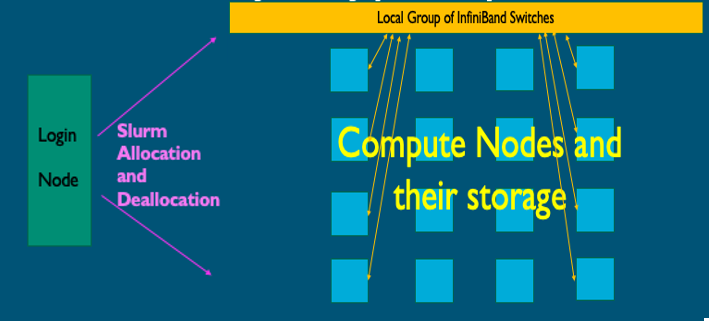
\includegraphics[width=\columnwidth]{images/cluster_layout.png}}
  \caption{Planned Burst-Buffer Architecture}
  \label{fig:cluster_layout}
\end{figure}

Our production private BeeOND filesystem  architecture was completed as shown in figure \ref{fig:cluster_layout}.  Slurm aided us in providing data locality to allocated job runs with Slurm partition information on our filesystem topology and the fact that Slurm has a built-in affinity for contiguous node allocation. 

Slurm provides useful run-time variable information that is passed through the Slurm function \textit {slurmstepd}.  In our implementation, we wanted to provide HPC users with the ability to toggle on-and-off usage of the BeeOND filesystem.  This was designed into our Slurm Prolog script with a Slurm variable using the Slurm 'Constraint' feature.  In our Slurm Prolog script, the batch variable \textit{SLURM\_JOB\_CONSTRAINTS} was checked for the value \textit{beeond}. If the constraint \textit{beeond} value was set, a log message was passed to standard node logging to reflect that a private BeeOND filesystem was user requested and was being used. 

We wanted each node in the BeeOND filesystem to know the role it had in the collective parallel filesystem.  Notification of the individual compute nodes was accomplished with the Slurm allocation variable \textit {SLURM\_NODELIST}. Passing \textit {SLURM\_NODELIST} inside Slurm Prolog with \textit{hostlist} allowed our Prolog script parser to determine the individual filesystem roles of the compute node in the node-local BeeOND filesystem. In our implementation, the \textit {SLURM\_NODELIST} variable was copied to an internal variable in each parallel Slurm Prolog script.  Once the internal variable was loaded with the variable value of Slurm allocated nodes, \textit {hostlist} was used to deconstuct the variable into a parsable compute node list.  Next, the hostname of the compute node was checked against the compute node list.  Using pre-determined architectural decisions, roles were assigned to each compute node in the Slurm allocation and services were started to create the BeeOND filsystem.

\subsection{Customized BeeOND Filesystem Management with Parameter Passing}

As part of the design of our BeeOND filesystem, we separated out the BeeOND filesystem management into separate start and stop scripts that were called by the Slurm Prolog and Epilog scripts.  The advantage of separate  management scripts was that we found that we could create more versatility in our filesystem architecture in future deployments on other HPC systems.  Also, we like the fact that we would have modularity in our start and stop functions to help us with software debugging.  

We wanted our BeeOND filesystem storage to be optimized for many different HPC architectures and different quantities of metadata and storage servers.  Through careful analysis of the pre-packaged BeeOND shell scripts \textit{beeond start} and the \textit{beeond stop} scripts, we discovered that the key pieces of the pre-packaged BeeOND start-up script consisted of initialization and stoppage of just a few filesystem component services.  With the knowledge that we gained from our script study, we were able to write our own custom BeeOND filesystem management software that fulfilled our needs for automatic filesystem composition and decomposition.  Further, our custom start and stop scripts provided us complete versatility in quantity of MDT and OST services and node placement.  

With our new custom scripts, in our BeeOND implementation, a Mangement server (Mgmt) component was the first service to run.  Mgmt calls were completed with a \textit {Mgmtd} storage directory, log file info, PID file, connection port, and as a daemon.  We chose the lowest node in each \textit {SLURM\_NODELIST} to be the Mgmtd server.

The second BeeOND filesystem component in our BeeOND filesystem  was the storage server.  Every BeeOND filesystem consists of even striping of data across a user-defined quantity of OSTs.  For our first BeeOND implementattion, we decided to make every node in our allocation a single OST on a local OSS server.  Each storage server call requires a Storage Store directory, log file information, a PID file, the Mgmtd connection port, the name of the Mgmtd server, and as a daemon. 

Again, the lowest entry in the \textit{SLURM\_NODELIST} became the default Metadata sever for our usage.  We did implement inherent capabilities into our custom scripting to allow us to alter the number of Metadata servers and placement of the servers, if we would like to modify those options, in the future.  Provided in our Metadata server start-ups are the name of the Mgmtd server, a Meta Store directory, log file information, a connection port, and daemonization.

Each node was a client of the node-local BeeOND parallel filesystem.  BeeOND implements the mount with the use of a \textit{helperd} service.  Provided to \textit{helperd} was the name of the Mgmtd server and the connection port.  Once the \textit {helperd} service was started, a \textit{beeond\_mount} command was called and the private BeeOND filesystem was mounted to /mnt/beeond.  
 
The final architectural layout of the node-local BeeOND filesystem is shown in figure \ref{fig:Node_local_storage_layout}.  The lowest node in the allocation became the Mgmt server, the Metadata server, an OST, and a client.  The other nodes in the Slurm allocation became both OST servers and clients.

\begin{figure}[!htb]
  \centerline{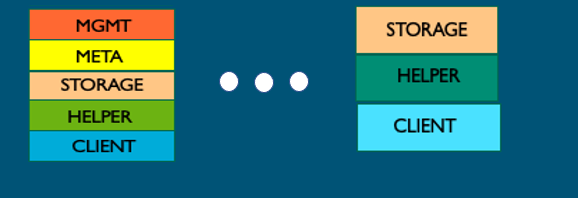
\includegraphics[width=\columnwidth]{images/Node_local_storage_layout.png}}
  \caption{Node Local Burst Buffer Architecture}
  \label{fig:Node_local_storage_layout}
\end{figure}

%\textbf{\textit{SLURM\_JOB\_CONSTRAINTS}} 

Once an HPC allocation was completed, the BeeOND filesystem process components were matched to each node-local storage mount using the same methods that were used in the Slurm Prolog scripts. After node identification, as part of the Slurm Epilog script, parameters were passed to an individual BeeOND stop script on every node in the private BeeOND filesystem.  A kill signal was sent to each compute node with a fuser command.  A polling check insured that the processes were stopped before an XFS reformat to the node-local file storage. After any BeeOND processes were stopped, the back-end XFS storage was reformatted and remounted for use in another potential Slurm allocation.

\subsection{Production HPC System Installation}

%Our first implementation of the new node-local BeeOND filesystem was on an ARM64 HPC system\ref{fig:Apollo70}.  The system consisted of a dual socket ThunderX2 processor with Socket Direct Nvidia/Mellanox 100 Gb/s EDR InfiniBand HCA ports and switches.  Each node contained a 1 TB SATA interface SSD (HPE Part Number: 875852-001).  The SSD was formatted with an XFS filesystem back-end.

Our first implementation of the new node-local private BeeOND filesystem design was on an ARM64 HPC system.  The system consisted of a dual socket ThunderX2 processor with Socket Direct Nvidia/Mellanox 100 Gb/s EDR InfiniBand HCA ports and switches.  Each node contained a 1 TB SATA interface SSD (HPE Part Number: 875852-001).  

%\begin{figure}[!htb]
%  \centerline{\includegraphics[width=\columnwidth]{images/Apollo70.png}}
%  \caption{HPE Apollo 70 Compute Node}
%  \label{fig:Apollo70}
%\end{figure}

We created a single 894GB partition on each SSD drive and formatted the drive as an XFS block device.  The BeeOND filesystem requires that the underlying block device support extended attributes. XFS filesystem provides extended attributes and is the standard filesystem for Red Hat 7.x and Red Hat 8.x Operating Systems.  As part of preparing each SSD block device for BeeOND use, we wrote a special UDEV rule that examined the partitions on the SSD device to make sure that only a single continuous partition of 894GB was on the device.  Next, our UDEV rule would assign the expected SSD, on \textit{/dev/sda1} to read/write permissions and create a symbolic device \textit{/dev/beeond\_store} to denote success of the readiness of the device for our node-local BeeOND filesystem block storage.  In the event of a failure of the UDEV rule, the compute node would not be put into Slurm queue and would be listed as not available.  

Our Production HPC systems use custom \textit{nodeup} and \textit{nodedown} scripts to examine the compute nodes for hardware and software issues, prepare the compute nodes for Slurm allocations, and prepare the compute node shared storage mounts.  We added our BeeOND node-local compute node mounts and the \textit{beeond} device driver management to the custom scripts.  In the event of a device driver mismatch to the kernel, BeeOND can do run-time re-compiling of the kernel module.  We incorporated the recompiling feature into our node initialization script.  Finally, the scripts mounted \textit{/dev/beeond\_store} on mount \textit{/beeond} readying the SSD for our node-local filesystem.


\section{Conclusions and Future Work}
Current HPC systems are limited in performance and architecture by the the stranding of disaggregated components. In current HPC systems, common tools do not exist to manage increasingly diverse network fabrics and component resources, such as, CPUs, hierarchical memory components, remote NVMe, and accelerators.  Due to lack of access to good Resource Management tools, current HPC systems suffer from inefficient over-design where resources must be provided locally, often in node, to make In instances that HPC running jobs could potentially require the resources.  In addition, the inability to dynamically share available resources, as they are required by running batch jobs can lead to reduced and inefficient computational performance and running job failure.  Centralized resource management can potentially mitigate, out-of-memory conditions, IO thashing, stranding of available resources, such as, CPUs, GPUs, and memories, and provide dynamic network fail-over.  It is clear that Resource Management, using a standardized interface, can enable clients to monitor, compose, and intelligently provision resources, in beneficial ways.

The OpenFabrics Management Framework (OFMF) is a open-source Resource Manager being developed by the OpenFabric Alliance (OFA), in partnership with the DMTF, SNIA, and the CXL Consortium. The OFMF implements Redfish and Swordfish through the implementation of a Swordfish Endpoint Emulator and network Agents.  The Emulator provides centralized resource monitoring and command control for the attached hardware resources and network fabrics, through matching network Agents. A Composability Manager, integrated with the OFMF, can mitigate stranded resources by providing a method for sharing hardware, CPUs, GPUs, NVM, and memories.  Integration with the OFMF provides the capability for dynamic provisioning of resources to maintain running client computations.  

In this paper, we described the OFMF architecture which enables composing platforms through management of network fabrics, storage fabrics, memory fabrics, and provisioning of GPUs, and CPU components.  The OFMF is designed for configuring fabric interconnects and managing composable disaggregated resources in dynamic HPC infrastructures using client-friendly abstractions.  The goal of the OFMF is to enable interoperability through common interfaces to enable client Managers to efficiently connect workloads with resources in a complex heterogenous ecosystem without having to worry about the underlying network technology.  

We illustrated the composability layer {}, the Redfish RESTful API {}, the OFMF services, and the design of a sample Agent. 

In conclusion, we are developing a solution to enable HPC ecosystems to move from statically defined infrastructure to dynamically defined infrastructure where workload resources can be provisioned depending upon workload needs yto provide the corredct resources to right applications at the right times.

The OFMF is capable of interfacing with multiple fabric managers by means of a set of agents in charge of translating vendor specific APIs into RedFish.



\bibliographystyle{plain}
%\bibliography{COMPSYS23}

\begin{thebibliography}{20}

\bibitem{beowulf}
  Beowulf Cluster,
  url = "https://en.wikipedia.org/wiki/Beowulf_cluster",
  note = "[Online: Accessed: Feb 1, 2023]".

\bibitem{eere}
  Data Centers and Servers - Buildings,
  url = "https://www.energy.gov/eere/buildings/data-centers-and-servers",
  2021.
  
\bibitem{dw}
  Deutsche Welle,
  Data centers keep energy use steady despite big growth,
  url="https://www.dw.com/en/data-centers-energy-consumption-steady-despite-big-growth-because-of-increasing-efficiency/a-60444548",
  January 24, 2022.
  
\bibitem{vmware}
  WMware,
  VMware : Why Energy Sobriety Should Be Top of Mind for Every Business Leader This Year,
  url="https://www.marketscreener.com/quote/stock/VMWARE-INC-58476/news/VMware-Why-Energy-Sobriety-Should-Be-Top-of-Mind-for-Every-Business-Leader-This-Year-42823597/"
  01/26/2023
  
\bibitem{fuzzball}
  CtrlIQ Fuzzball,
  url="https://ciq.co/products/fuzzball/hpc/",
  2023.
  
\bibitem{flux}
  Flux:  A Fully Hierarchical Workload Manager for Supercomputing,
  url="https://ipo.llnl.gov/sites/default/files/2022-02/Flux_RD100_Final.pdf",
  2023. 
  
\bibitem{reportlinker}
  Composable Infrastructure Market by Type, Vertical And Region - Global Forecast to 2023,
  url="https://www.reportlinker.com/p05620908/Composable-Infrastructure-Market-by-Type-Vertical-And-Region-Global-Forecast-to.html",
  2018.
  
\bibitem{liquid}
  Liqid touts composable infrastructure at Dell Technologies World,
  url="https://venturebeat.com/data-infrastructure/liqid-touts-composable-infrastructure-at-dell-technologies-world/",
  May 3, 2022.
  
\bibitem{gigaio}
  url="https://gigaio.com/",
  note = "[Online: Accessed: Feb 1, 2023]". 
  
\bibitem{liqidmf}
  Liqid introduces multi-fabric support for composable infrastructure,
  url = "https://www.itopstimes.com/itops/liqid-introduces-multi-fabric-support-for-composable-infrastructure/",
  April 29th, 2019.
  
\bibitem{cdi}
  Composable disaggregated infrastructure,
  url = "https://en.wikipedia.org/wiki/Composable_disaggregated_infrastructure",
  note = "[Online: Accessed: Feb 1, 2023]".

\bibitem{whatcdi}
  What is composable infrastructure?,
  url="https://www.networkworld.com/article/3266106/what-is-composable-infrastructure.html",
  MAR 27, 2018.

\bibitem{fungible}
  Fungible, Inc.,
  url = "https://en.wikipedia.org/wiki/Fungible_Inc.",
  note = "[Online: Accessed: Feb 1, 2023]".


\end{thebibliography}
\end{document}
